%!TEX root = ../thesis.tex
\chapter{Context generalisation}

\label{ch:Context}

Structures such as \smap{} and \ifop{}, which alter control flow are not compatible with the \yauhau{} base transformation.
In the preceding Chapters we have learned how both these structures may be altered individually to extract a particular node from them.
However these structures do not occur exclusively independent, rather they may be nested into one another in arbitrary fashion.
The transformations as described in the previous chapters are only able to extract selected nodes from one particular, single layer of one of these structures.
I.e. the \smap{} transformation\footnote{A slightly modified version of the transformation} moves all fetch nodes from one \smap{} into the next outer layer.

When designing the unified control flow rewrite I realised however that as long as one possesses a rewrite for each type structure which extracts nodes from exactly one level we can build an algorithm which uses these individual rewrites to extract \emph{all} nodes from \emph{all} contexts in a semantics preserving way.

\begin{figure}
\begingroup
\definecolor{green(html/cssgreen)}{rgb}{0.0, 0.5, 0.0}
\catcode`\@=\active
\def@#1@{\textcolor{green(html/cssgreen)}{#1}}
\begin{minted}[escapeinside=||]{Clojure}
(|@defalgo@| algo1 [param]
  (smap
    (|@algo@| [val]
      (if (is-iterable? val)
        (smap (|@algo@| [item] (compute-something (fetch item)))
          val)
        (some-operation val))))
\end{minted}
\endgroup
\caption{Nested context example}
\label{fig:nested-context-example}
\end{figure}

\begin{figure}
    \includegr{context-nesting-example-exploded}
    \caption{Visual example of context nesting with exploded stack}
    \label{fig:visual-context-nesting-example-exploded}
\end{figure}

\section{Definition}

In order to talk about structures such as \smap{} and \ifop{}, in particular for the purposes of our unified extraction algorithm we introduce a new concept to Ohua called \emph{context}.
\emph{Contexts} are a much broader concept than just \ifop{} and \smap{} but this is where the idea first emerged.
Contexts now solve an issue emerging from the internal representation of the program.
The information in a dataflow graphs is limited to data dependencies and derivable properties.
However real programs have properties which do not emerge structurally in a dataflow graph.
Control flow structures such as \smap{} and \ifop{} for instance change the properties of the contained subgraph but this is not structurally visible in the graph.
In order to determine whether a certain node has such properties we need to look and interpret the actual labels of the nodes.
In the example in Figure~\ref{fig:visual-context-nesting-example-exploded} these properties are marked with dotted circles, because they are not inherently visible from the structure of the graph itself.

\emph{Context} is the general name we give these not structurally emergent properties of a subgraph.
The context type is a label which refers to the behaviour of that particular context, i.e. \ifop{} or \smap{}.
An instance of a context is a concrete subgraph of the dataflow graph, as seen in Figure~\ref{fig:visual-context-nesting-example-exploded}.
In this figure you can also see the typical enter and exit nodes of a context, which are located at the context boundary.
The type of enter and exit nodes determines the behaviour of the context itself.

\subsection{The stack}

A context stack $S(n)$ is a ordered list of nested contexts a node is contained in.
In the following paragraphs I will sometimes speak of a context and sometimes of a context stack.
Both are equivalent, since every context can be uniquely associated with a context stack and vice versa.
The context associated with a stack $s$ is the topmost context of $s$.
The stack associated with a context $c$ is the context stack of its exit node.
See also Figure~\ref{fig:visual-context-nesting-example-exploded}.

\subsubsection{Notation}

\begin{tabular}{c | l}
  Symbol & Semantics \\ \hline
  $c \rightarrow_{pop} c'$ & Removing the topmost element from the stack $c$ yields $c'$ \\
  $c \rightarrow_{pop}^n c'$ & Removing the topmost $n$ elements from the stack $c$ yields $c'$ \\
  $c \rightarrow_{pop}^* c'$ & Removing an unspecified amount of entries from the top of $c$ yields $c'$ \\
\end{tabular}

\subsubsection{Definitions}

If there are two context stacks $s_1$ and $s_2$ and the successive removal of elements from the top of $s_1$ yields $s_2$, then we say $s_1$ is \textit{nested} in $s_2$ or a \emph{child context} of $s_2$ and $s_2$ is a \textit{subcontext} or \emph{parent context} of $s_1$.

\[
  s_1 \rightarrow_{pop}^n s_2 \mid n > 0
\]

A root context $r$ is the context of the empty context stack $r = []$.
The amount of elements $D(s)$ which need to be removed from a stack $s$ to reach the root context is its \emph{nesting depth}, which equates to the height of the stack.

\[
  D(s) := s \rightarrow_{pop}^d r
\]

Truncating $T_n(s)$ a stack $s$ to $n$ means to remove elements from the top until a nesting depth of $n$ is reached.
If the nesting of the original stack was already lower than $n$ the truncated stack is the original stack itself.

\[
  T_n(s) :=
  \begin{cases}
    s' \mid s \rightarrow_{pop}^* s', D(s') = n & D(s) > n \\
    s & D(s) \leq n \\
  \end{cases}
\]

Context effects aggregate in a context stack.


\subsubsection{Properties}

There are a few general properties which can be asserted about contexts in the Ohua sense.

\begin{itemize}
  \item \textbf{Contexts are naturally fully enclosing.}
        This means that in a valid program\footnote{On the level of dataflow operators one might be able to construct graphs which contain partially overlapping contexts, however the resulting program would be invalid in that it breaks some invariants and most likely either not execute or never terminate.} two contexts never partially overlap.
        Truncating both to the length of the smaller stack either yields the same stack for both or one were no element occurs in both stacks.
        Formally
        \[
        \forall s_1, s_2 | n = \min(D(s_1), D(s_2)) :=
          \begin{cases}
            T_n(s_1) = T_n(s_2) \\
            e_{s_1} \neq e_{s_2} \mid e_{s_1} \in T_n(s_1), e_{s_2} \in T_n(s_2) \\
          \end{cases}
        \]
        An example of this property can be seen in Figure~\ref{fig:visual-context-nesting-example-exploded}.
        Every context is completely embedded within any of its parent contexts.

  \item \textbf{Contexts are an inherited property.}
        Nodes which are not special, context changing nodes such as \smap{} or \texttt{ifThenElse} inherit their context from their preceding nodes.
        Briefly said a node N is in every context any of its preceding nodes is in.
        Since, as mentioned above, contexts do not partially overlap, contexts of preceding nodes are always subcontexts of one another.
\end{itemize}

Contexts are special in Ohua because as of yet they are exclusively builtin and cannot be user defined.

\section{Detection}

\subsection{IR Based}

There are mutliple ways of detecting the context at various stages of the compiler
This algorithm employes a strategy whereby the IR graph would be traversed in topological order.
Each nodes context would be calculated from the maximal context out of the contexts from the preceding nodes (see inheritance property).
Maximal context here means the most deeply nested (see full enclosure property).
Then depending on the type of node this context stack would be transformed.

\begin{enumerate}
  \item If the node opens a new context (\smap{}, \ifop{}) a new frame for that context is pushed onto the context stack.
  \item If the node closes the current topmost context (\texttt{collect}, \texttt{select}) the topmost frame is popped off the stack.
  \item If the node neither closes nor opens a new context stack remains the same.
  \item If the node closes a context which is not the current topmost context an error os thrown.
\end{enumerate}

The node would then be labeled with the transformed context stack.

\subsection{Source based}

Alternatively context detection can be performed during the AST traversals on the source code.
This subgraphs of the context are now easier to find as they are just a subtree in the AST.
Currently in Ohua context detection is done on the AST, when the Clojure code is being transformed into the IR, see Figure~\ref{fig:ohua-compiler-flow-with-ctx}.

\begin{figure}
  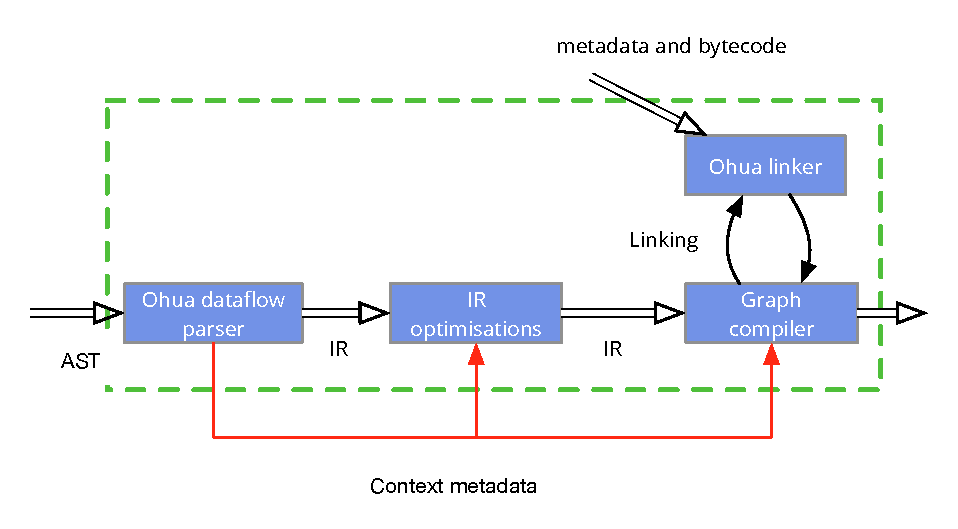
\includegraphics[width=\textwidth]{ohua-compiler-flow-with-ctx}
  \caption{Context information in the Ohua compiler flow}
  \label{fig:ohua-compiler-flow-with-ctx}
\end{figure}

\begin{figure}
  \includegr{context-pointers}
  \caption{Visualisation of context pointers after the AST traversal}
  \label{fig:context-pointers}
\end{figure}

At this point the subgraphs enclosed by the context are even more easily visible.
When we traverse the AST and we encounter a context introducing function like \smap{}, we mark the enclosed function such that when it is being traversed all nodes inside are annotated with a reference to the \smap{} starting node.
This overwrites any previous marker.
What we end up with, as a result, is an IR, where every node has, in its metadata, a reference to its closest context starting node, a visual representation from our example of the nested contexts from earlier can be found in Figure~\ref{fig:context-pointers}.
The context starting node then has a reference to its nearest outer context and thus we can rebuild the entire context stack for each node afterwards.
For this we use dynamic programming by populating a HashMap with the stacks for each node, reusing previously computed results.
This can be done safely because Clojure standard library data structures like \texttt{Vector} are immutable and therefore safe to reuse.
After this process is completed we obtain a Map from node ids to completely resolved context stacks which is handed to subsequent transformations.

\section{Unwinding nested context}

Contexts like \ifop{} and \smap{} can be arbitrarily nested and interleaved in a program.
The detection algorithm, as described above, is able to correctly identify stacks of contexts for each node of the graph.
Subsequently we would like to `undo' each layer of context around each fetch to guarantee the node is only executed once per program run, which allows us to batch it.
This `undoing' operation should be reasonably efficient and yet easy to understand.

My context unwinding algorithm, which combines the \ifop{} and \smap{} transformations to deal with arbitrary nesting, uses the properties of contexts as mentioned above.
It unwinds one context at a time, dispatching to the appropriate handler, see Figure~\ref{fig:yauhau-rewrite-flow}, starting with the deepest nesting level.
This unifying unwinding algorithm is not limited to \ifop{} and \smap{} contexts, but can be configured as to the type of contexts it dispatches on.
The reason this results in a correct unwinding is that if a particular context has been unwound around a particular fetch, this fetch now lies in what was formerly the parent context.
Since this parent context cannot have been as deeply nested as the now unwound child context, it itself has not been unwound yet since we go from high nesting to low nesting.
At the same time since all contexts are eventually being unwound the parent context has already been scheduled for unwinding.
Through this iterative unwinding all contexts around fetches are eventually unwound completely.

The correct order is achieved by using a work list of contexts to unwind.
The list is obtained by collecting the set of all context stacks on fetches, adding all substacks, ordering by length and finally mapping to the topmost element of the stack.
This last list is guaranteed to have no duplicates, due to the ``fully enclosed'' property of contexts.

In order to be as efficient as possible transformations are performed in a stateful way.
Individual transformation algorithms insert and delete nodes from the graph, insert and delete edges, as well as alter contexts for existing nodes or label new nodes with appropriate contexts.
Currently no sanity checks for the validity of those alterations are present, therefore the individual transformations themselves are responsible for preserving the integrity of the graph and its associated metadata structures.
This is not a hard limitation and might change in the future if we decide to allow more or user defined rewrites.
